\documentclass[14pt]{extarticle}
% Full article preamble (duplicated, no common file)
\usepackage{fontspec}
\usepackage[a4paper,margin=2.5cm,includefoot]{geometry}
\usepackage{polyglossia}
\usepackage{amsmath}
\usepackage{amssymb}
\usepackage{xcolor}
\usepackage{fancyhdr}
\usepackage{graphicx}
\usepackage{listings}
\usepackage[most]{tcolorbox}
\usepackage{pifont}
\usepackage{enumitem}
\usepackage{titlesec}
\usepackage[bottom]{footmisc}
\usepackage{titling}
\usepackage{minted}
\usepackage{etoolbox}
\usepackage{array}
\usepackage{extsizes}

\newfontfamily\emoji{Segoe UI Emoji}

\pagestyle{fancy}

\setmainlanguage[numerals=western]{arabic}
\setotherlanguage{english}
\newfontfamily\arabicfont[Script=Arabic]{Amiri}
\newfontfamily\arabicfonttt[Script=Arabic]{Courier New}

\lstset{
  language=[Sharp]C,
  numbers=left,
  stepnumber=1,
  numbersep=8pt,
  frame=single,
  basicstyle=\ttfamily\small,
  keywordstyle=\color{blue},
  stringstyle=\color{red},
  commentstyle=\color{green!50!black}
}

\newif\ifdetailed
\ifdefined\setdetailed
  \setdetailed
\fi

\newif\ifwithsols
\ifdefined\setwithsols
  \setwithsols
\fi

% unified tcolorboxes for articles
\tcbset{colback=white, colframe=black, fonttitle=\bfseries, boxrule=0.8pt}
\newtcolorbox{boxDef}[1][]{colback=blue!5!white,colframe=blue!75!black,
  title={{\emoji📘} تعريف\ifx\\#1\\\else ~#1\fi :}}
\newtcolorbox{boxExercise}[1][]{colback=cyan!5!white,colframe=cyan!70!black,
  title={{\emoji🧩} تمرين\ifx\\#1\\\else ~#1\fi :}}
\newtcolorbox{boxExample}[1][]{colback=yellow!5!white,colframe=orange!90!black,
  title={{\emoji📝} مثال\ifx\\#1\\\else ~#1\fi :}}
\newtcolorbox{boxNote}[1][]{colback=gray!10!white,colframe=black,
  title={{\emoji✨} ملاحظة\ifx\\#1\\\else ~#1\fi :}}
\newtcolorbox{boxAttention}[1][]{colback=magenta!10!white,colframe=magenta!80!black,
  title={{\emoji🔔} تنبيه\ifx\\#1\\\else ~#1\fi :}}
\newtcolorbox{boxWarning}[1][]{colback=red!5!white,colframe=red!75!black,
  title={{\emoji⚡} ملاحظة هامة\ifx\\#1\\\else ~#1\fi :}}
\newtcolorbox{boxSolution}[1][]{colback=green!5!white,colframe=green!60!black,
  title={{\emoji✅} حل\ifx\\#1\\\else ~#1\fi :}}
\newtcolorbox{boxSymbol}[1][]{colback=purple!5!white,colframe=purple!70!black,
  title={{\emoji🔣} رمز\ifx\\#1\\\else ~#1\fi :}}

\tcbset{simplecode/.style={ colback=gray!5, colframe=black!50, boxrule=0.4pt, arc=2pt, left=4pt,right=4pt,top=4pt,bottom=4pt}}
\newenvironment{boxCode}{\begin{tcolorbox}[simplecode]}{\end{tcolorbox}}

\newcolumntype{C}[1]{>{\centering\arraybackslash}p{#1}}

% redefine spaces after titles
\makeatletter
\renewcommand{\@maketitle}{%
  \begin{center}
    {\huge \bfseries \@title \par}%
    \vskip 0.2em % space between title and author
    {\large \@author \par}%
    % \vskip 0.2em % space between author and date
    % {\normalsize \@date \par}%
  \end{center}
}
\makeatother

\fancyhf{} % clear default
\fancypagestyle{plain}{
  \fancyhf{}
  \fancyhead[L]{مدرسة التسامح الشاملة}
  % \fancyhead[L]{
\includegraphics[height=1cm]{../../../images/logoTasamoh.png}}
  \fancyhead[R]{الأستاذ محمود اغبارية}
  \fancyfoot[C]{\thepage}
}

\fancyhead[L]{مدرسة التسامح الشاملة}
\fancyhead[R]{الأستاذ محمود اغبارية}
\fancyfoot[C]{\thepage}
% \date{\today}

\setcounter{tocdepth}{3} % only section subsection and subsubsection in TOC


% ----------------------


% \begin{document}

% \maketitle

% % \clearpage  % start TOC on a new page
% % \renewcommand{\contentsname}{جدول المحتويات}
% % \tableofcontents
% % \clearpage

% \part*{part 1} % the * prevents numbering
% \section*{مقدمة}
% \subsection*{مثال رياضي}
% \subsubsection*{مثال فرعي}
% \paragraph*{ paragraph 1}
% \subparagraph*{sub paragraph 1}

% \ifdetailed
% \begin{english}
% \begin{minted}{csharp}
% // C# Example
% \end{minted}
% \end{english}
% \fi

% OLD WAY
% \ifdetailed
% \begin{english}
% \begin{lstlisting}
% // C# Example
% \end{lstlisting}
% \end{english}
% \fi

% % 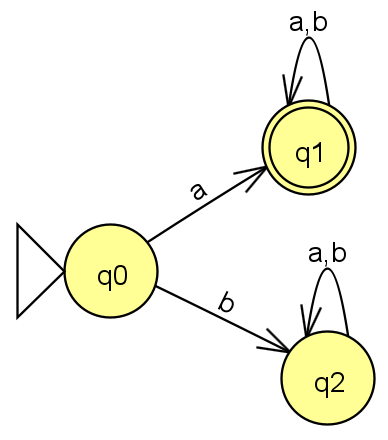
\includegraphics[width=0.2\textwidth]{../../../images/DFAs/ex1_q1.png}



% \vspace{3cm}
% \begin{flushleft}
% أرجو لكم وقتًا ممتعًا.

% الأستاذ محمود اغبارية.
% \end{flushleft}


% \end{document}


\title{اختبار خفيف للصف 10-10}

\begin{document}
\maketitle

\begin{enumerate}[itemsep=1.8em]

\item
أي من التالية هي \textbf{عملية خارجية تتلقى عددًا عشريًا وتعيد عددًا صحيحًا}؟
\begin{english}
\begin{enumerate}[label=(\alph*)]
    \item public static int Foo(double x)
    \item public static double Foo(int x)
    \item public static int Foo()
    \item public static double Foo()
\end{enumerate}
\end{english}
\ifwithsols
\begin{boxSolution}
الإجابة: (a).
تُعيد \textenglish{int} وتتلقى \textenglish{double}.
\end{boxSolution}
\fi

% -------------------------------

\item
أي من التالية هي \textbf{عملية خارجية تستقبل عددًا عشريًا}؟
\begin{english}
\begin{enumerate}[label=(\alph*)]
    \item public static void Foo(double x)
    \item public static double Foo()
    \item \begin{minted}{csharp}
public static void Foo()
{
    double d = double.Parse(Console.ReadLine());
}
\end{minted}
    \item public static double Foo(double d)
\end{enumerate}
\end{english}
\ifwithsols
\begin{boxSolution}
الإجابة: (c).
"تستقبل" تعني أنّ العملية تقرأ من المستخدم داخلها.
\end{boxSolution}
\fi

% -------------------------------

\item
أي من التالية هي \textbf{عملية لا تتلقى شيئًا ولا تعيد شيئًا}؟
\begin{english}
\begin{enumerate}[label=(\alph*)]
    \item public static void Foo()
    \item public static int Foo(int x)
    \item public static void Foo(int x)
    \item public static int Foo()
\end{enumerate}
\end{english}
\ifwithsols
\begin{boxSolution}
الإجابة: (a).
لا بارامترات ولا return.
\end{boxSolution}
\fi

% -------------------------------

\clearpage
\item
أي من التالية هي \textbf{عملية تتلقى نصًا وتعيد نصًا جديدًا}؟
\begin{english}
\begin{enumerate}[label=(\alph*)]
    \item public static string Greet(string name)
    \item public static void Greet()
    \item public static void Greet(string name)
    \item public static string Greet()
\end{enumerate}
\end{english}
\ifwithsols
\begin{boxSolution}
الإجابة: (a).
تتلقى \textenglish{string} وتعيد \textenglish{string}.
\end{boxSolution}
\fi

% -------------------------------

\item
أي من التالية هي \textbf{عملية تستقبل عددًا صحيحًا وتعيد عددًا صحيحًا}؟
\begin{english}
\begin{enumerate}[label=(\alph*)]
    \item public static int Square(int n)
    \item \begin{minted}{csharp}
public static int Square()
{
    int n = int.Parse(Console.ReadLine());
}
\end{minted}
    \item public static void Square(int n)
    \item public static void Square()
\end{enumerate}
\end{english}
\ifwithsols
\begin{boxSolution}
الإجابة: (b).
تقرأ العدد من المستخدم ثم تعيده.
\end{boxSolution}
\fi

% -------------------------------

\item
أي من التالية تعريف صحيح لعملية \textbf{تُعيد قيمة منطقية (bool)} وتستقبل عددًا صحيحًا؟
\begin{english}
\begin{enumerate}[label=(\alph*)]
    \item public static bool IsEven(int n)
    \item public static void IsEven(int n)
    \item public static int IsEven(bool n)
    \item \begin{minted}{csharp}
public static bool IsEven()
{
    int n = int.Parse(Console.ReadLine());
}
\end{minted}
\end{enumerate}
\end{english}
\ifwithsols
\begin{boxSolution}
الإجابة: (a).
نوع الإرجاع \textenglish{bool} وتستقبل \textenglish{int}.
\end{boxSolution}
\fi

% -------------------------------
\clearpage
\item
أي من التالية هي \textbf{عملية خارجية تتلقى ولا تعيد}؟
\begin{english}
\begin{enumerate}[label=(\alph*)]
    \item public static void Foo(int n)
    \item public static int Foo()
    \item public static int Foo(int n)
    \item public static string Foo()
\end{enumerate}
\end{english}
\ifwithsols
\begin{boxSolution}
الإجابة: (a).
تتلقى عددًا صحيحًا ولا ترجع شيئًا.
\end{boxSolution}
\fi

% -------------------------------

\item
أي من التالية هي \textbf{عملية خارجية تُعيد ولا تتلقى}؟
\begin{english}
\begin{enumerate}[label=(\alph*)]
    \item public static int GetNumber()
    \item public static void PrintNumber(int n)
    \item public static int GetNumber(int n)
    \item public static void GetNumber()
\end{enumerate}
\end{english}
\ifwithsols
\begin{boxSolution}
الإجابة: (a).
لا بارامترات وتُعيد قيمة.
\end{boxSolution}
\fi

% -------------------------------

\item
أي من التالية هي \textbf{عملية تُعيد عددًا عشريًا}؟
\begin{english}
\begin{enumerate}[label=(\alph*)]
    \item public static double GetAverage(int a, int b)
    \item public static int GetAverage(double a, double b)
    \item public static void GetAverage(double a, double b)
    \item public static string GetAverage(int a, int b)
\end{enumerate}
\end{english}
\ifwithsols
\begin{boxSolution}
الإجابة: (a).
نوع الإرجاع \textenglish{double}.
\end{boxSolution}
\fi

% -------------------------------

\clearpage
\item
أي من التالية هي \textbf{عملية خارجية لا تتلقى ولكنها تستقبل عددًا عشريًا وتعيده}؟
\begin{english}
\begin{enumerate}[label=(\alph*)]
    \item public static double Foo(double x)
    \item \begin{minted}{csharp}
public static double Foo()
{
    double d = double.Parse(Console.ReadLine());
    return d;
}
\end{minted}
    \item public static void Foo(double x)
    \item public static void Foo()
\end{enumerate}
\end{english}
\ifwithsols
\begin{boxSolution}
الإجابة: (b).
تقرأ من المستخدم وتعيد القيمة.
\end{boxSolution}
\fi

% -------------------------------

\item
معطاة العملية:
\begin{english}
\begin{minted}{csharp}
public static void Foo(string name, int age)
\end{minted}
\end{english}
أي من التالية هي طريقة الاستدعاء الصحيحة؟
\begin{english}
\begin{enumerate}[label=(\alph*)]
    \item string result = Foo("Majd", 10);
    \item Foo("Majd", 10);
    \item int result = Foo("Majd", 10);
    \item \begin{minted}{csharp}
string name = Console.ReadLine();
int age = int.Parse(Console.ReadLine());
Foo();
\end{minted}
\end{enumerate}
\end{english}
\ifwithsols
\begin{boxSolution}
الإجابة: (b).
عملية void تُستدعى مباشرة دون تخزين نتيجة.
\end{boxSolution}
\fi

% -------------------------------

\clearpage
\item
معطاة العملية:
\begin{english}
\begin{minted}{csharp}
public static int Add(int a, int b)
\end{minted}
\end{english}
أي من التالية صحيحة؟
\begin{english}
\begin{enumerate}[label=(\alph*)]
    \item Add(5, 10);
    \item int x = Add(5, 10);
    \item double x = Add(5, 10);
    \item \begin{minted}{csharp}
int a = 4;
int b = 8;
Console.WriteLine(Add);
\end{minted}
\end{enumerate}
\end{english}
\ifwithsols
\begin{boxSolution}
الإجابة: (b).
ترجع int لذا يجب حفظها في متغير من نفس النوع.
\end{boxSolution}
\fi

% -------------------------------

\item
معطاة العملية:
\begin{english}
\begin{minted}{csharp}
public static double Average(double x, double y)
\end{minted}
\end{english}
اختر الاستدعاء الصحيح:
\begin{english}
\begin{enumerate}[label=(\alph*)]
    \item double a = Average(4, 5);
    \item Average();
    \item Average(4);
    \item Average("4","5");
\end{enumerate}
\end{english}
\ifwithsols
\begin{boxSolution}
الإجابة: (a).
يجب تمرير قيمتين عشريتين وحفظ النتيجة في متغير double.
\end{boxSolution}
\fi

% -------------------------------

\clearpage
\item
أي من التالية تُظهر الفرق بين عملية \textbf{تستقبل} عددًا صحيح و\textbf{تتلقى} عددًا صحيحًا؟
\begin{enumerate}[label=(\alph*)]
    \item \begin{minted}{csharp}
void Foo()
int x = int.Parse(Console.ReadLine());
\end{minted}
    \item \begin{minted}{csharp}
void Foo(int x)
\end{minted}
    \item كلاهما صحيح لكن المعنى مختلف.
    \item لا فرق بينهما.
\end{enumerate}
\ifwithsols
\begin{boxSolution}
الإجابة: (c).
الأولى تستقبل من المستخدم، الثانية تتلقى بارامتر.
\end{boxSolution}
\fi

% -------------------------------

\item
ما الفرق بين العمليتين التاليتين؟
\begin{minted}{csharp}
public static void Foo(int n)
public static int Foo(int n)
\end{minted}
\begin{enumerate}[label=(\alph*)]
    \item الأولى لا تُعيد قيمة، الثانية تُعيد قيمة صحيحة.
    \item الثانية لا تُعيد قيمة، الأولى تُعيد قيمة صحيحة.
    \item الاثنتان متطابقتان.
    \item الأولى تُعيد قيمة نصية.
\end{enumerate}
\ifwithsols
\begin{boxSolution}
الإجابة: (a).
الفرق في نوع الإرجاع فقط.
\end{boxSolution}
\fi

% -------------------------------

\item
أي من التالية تعريف صحيح لعملية \textbf{تتلقى نصًا وتعيد طول النص}؟
\begin{english}
\begin{enumerate}[label=(\alph*)]
    \item public static int GetLength(string s)
    \item public static string GetLength(int s)
    \item public static void GetLength(string s)
    \item public static bool GetLength(string s)
\end{enumerate}
\end{english}
\ifwithsols
\begin{boxSolution}
الإجابة: (a).
تتلقى string وتُعيد int (طول النص).
\end{boxSolution}
\fi

% -------------------------------

\clearpage
\item
أي من التالية تعريف صحيح لعملية \textbf{تتلقى عددًا عشريًا وتعيد ما إذا كان موجبًا}؟
\begin{english}
\begin{enumerate}[label=(\alph*)]
    \item public static bool IsPositive(double n)
    \item public static double IsPositive(double n)
    \item public static void IsPositive(double n)
    \item public static bool IsPositive()
\end{enumerate}
\end{english}
\ifwithsols
\begin{boxSolution}
الإجابة: (a).
تُعيد bool وتستقبل double.
\end{boxSolution}
\fi

% -------------------------------

\item
أي من التالية هي \textbf{عملية خارجية تستقبل عددًا صحيحًا وتطبع مربعه فقط}؟
\begin{english}
\begin{enumerate}[label=(\alph*)]
    \item public static void PrintSquare(int n)
    \item public static int PrintSquare(int n)
    \item public static void PrintSquare()
    \item public static void PrintSquare(double n)
\end{enumerate}
\end{english}
\ifwithsols
\begin{boxSolution}
الإجابة: (a).
تطبع فقط لذا نوعها void وتتلقى int.
\end{boxSolution}
\fi

% -------------------------------

\item
أي من التالية هي \textbf{عملية خارجية لا تستقبل شيئًا وتُعيد عددًا ثابتًا}؟
\begin{english}
\begin{enumerate}[label=(\alph*)]
    \item public static int GetNumber()
    \item public static void GetNumber()
    \item public static double GetNumber(int x)
    \item public static string GetNumber()
\end{enumerate}
\end{english}
\ifwithsols
\begin{boxSolution}
الإجابة: (a).
لا بارامترات وتُعيد int.
\end{boxSolution}
\fi

% -------------------------------

\item
أي من التالية هي \textbf{عملية خارجية تُعيد عددًا عشريًا}؟
\begin{english}
\begin{enumerate}[label=(\alph*)]
    \item public static double Foo()
    \item public static int Foo()
    \item public static void Foo()
    \item public static string Foo()
\end{enumerate}
\end{english}
\ifwithsols
\begin{boxSolution}
الإجابة: (a).
نوع الإرجاع double.
\end{boxSolution}
\fi

\end{enumerate}

\end{document}
